% !TeX spellcheck = en_US

\chapter{System Design}
\label{ch:system}

\section{Distributed Architecture}
\label{sec:arch}

In this chapter, we are going to present technical details of our  \textit{Mono3d} solution.
We will start by laying out the high-level architecture, as displayed in Figure~\ref{fig:mono3d-highlevel}.

\begin{figure}[htb]
    \centering
    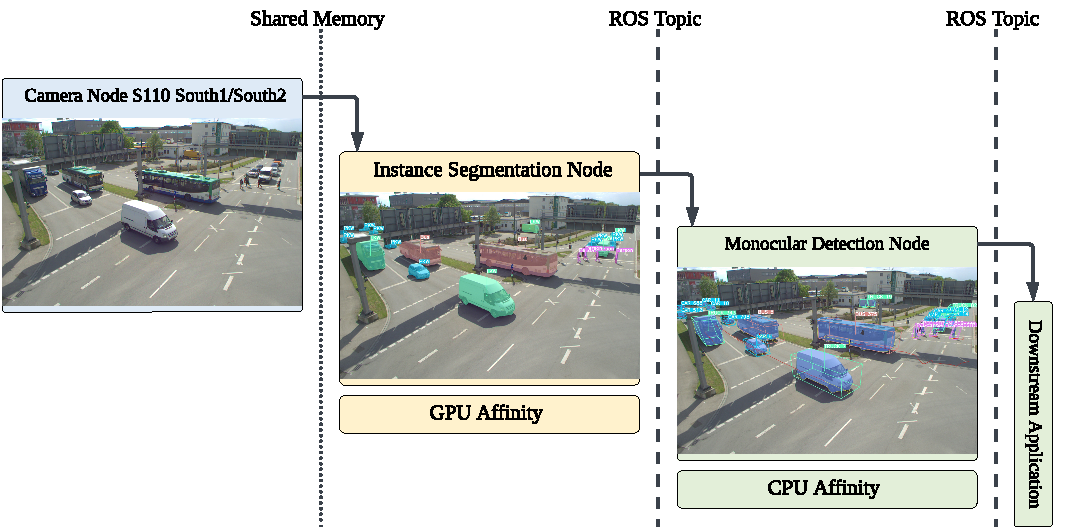
\includegraphics[width=\linewidth]{figures/mono3d-pipeline-highlevel}
    \caption{High-level sketch of the implemented \textit{Mono3d} solution. The Camera Driver Node publishes camera frames to Shared Memory. They are picked up from there by the $2D$ Instance Segmentation node, which requires a machine with strong GPU resources. The detected instances, including their instance masks, are published for each frame via \textit{ROS}, and received by the $3D$ detector node, which does not require a GPU.}
    \label{fig:mono3d-highlevel}
\end{figure}

We have divided our \textit{Mono3d} architecture into three independent process nodes.
A camera driver node, a $2D$ instance segmentation node, and a $3D$ detection node.
The camera driver node publishes full-resolution $1920p$ RGB image frames at $60Hz$, requiring a throughput of (roughly) $360 \text{MiB}$ per second.
This makes shared memory a good transport medium.
For our solution, we make use of the \textit{Eclipse eCAL} shared memory library \footnote{\hyperlink{https://eclipse-ecal.github.io/ecal/index.html}{https://eclipse-ecal.github.io/ecal/index.html}} to facilitate the communication of camera frames.
The frames are continuously received by the the $2D$ Instance Segmentation node, which is bottlenecked by the performance of the used GPU.
From there, the instance masks of detected objects are published to downstream processes via \textit{ROS}.
In this setup, the second stage our two-stage monocular $3D$ detector is just another consumer of the detected $2D$ instances \textemdash many other consumers may exist for different purposes.
In the second detector stage (the $2D \rightarrow 3D$ lifting stage), $2D$ instance detections are received via ROS and annotated with hypotheses regarding their $3D$ pose.
Again, via \textit{ROS}, these $3D$ detections are then broadcast to downstream applications, such as sensor fusion, visualization, or an autonomous vehicle.
This separation of the detection pipeline into multiple concurrent, networked processes offers numerous advantages:

\begin{enumerate}
    \item \textbf{Increased robustness}: A distributed multi-process solution enhances system robustness by enabling fault tolerance and redundancy.\ When a process fails or encounters an error, other processes in the system can continue to function, minimizing the impact of the failure.\ This capability to recover and adapt to faults makes the overall system more reliable, preventing single points of failure from causing widespread disruptions.
    \item \textbf{Separation of functional concerns}: In a distributed system, each process can focus on a specific functionality, promoting modularity and maintainability.\ This separation of concerns simplifies the design and development of the system, making it easier to understand, debug, and extend.\ It also facilitates reusability, as individual components can be easily replaced or integrated into other systems without affecting the overall system's functionality.
    \item \textbf{Improved assignment of hardware}: The networked solution allows for better resource allocation and hardware utilization.\ By spreading tasks across multiple processes and physical machines, the system can allocate specific resources, such as GPUs, to each process based on its requirements.\ This flexibility enables more efficient use of available hardware, reducing resource contention and potential bottlenecks, while also providing the opportunity to optimize cost and energy consumption.
    \item \textbf{Increased performance}: The asynchronous process collaboration enables parallelism, allowing multiple tasks to be executed concurrently.\ This parallel execution can significantly improve the overall performance and throughput of the system.\ By leveraging the processing capabilities of multiple machines, distributed systems can handle larger workloads and scale more effectively than a single-process system.\ Additionally, this architecture allows for load balancing, which can help distribute work evenly and prevent overloading individual components.
\end{enumerate}

Natural tradeoffs of this architecture are increased complexity and a nonzero communication overhead, as data must be serialized and deserialized into discrete messages.
However, the advantages of the distributed approach tend to outweigh the negatives, especially where scalability is a concern.

% ----------------------------------------------------

\section{The 2D Object Detector}
\label{sec:segmentation}

The $2D$ Object Detector receives camera input frames from a camera driver node via shared memory.
It uses an off-the-shelf Object Recognition and Instance Segmentation solution (currently \textit{YOLOv7/Blendmask}~\cite{wang2022yolov7, chen2020blendmask}) to detect $2D$ bounding boxes and pixel masks of Vehicles and Vulnerable Road Users (VRUs).
As the performance of such an object detection solution inversely scales to the square of the input image resolution, the $2D$ object detector may also downsize the incoming frames from $1920*1200$ to $1280*800$ or even $640*400$ using \textit{OpenCV}~\cite{opencv_library}.
The performance impact of this downscaling is further explored in Section~\ref{sec:performance}.
As the instance masks of detected objects must be efficiently passed via \textit{ROS} messages, bit packing~\cite{5219512} is used to efficiently serialize the pixel mask arrays for each instance.
Earlier work within Providentia~\cite{leonthesis} went so far as to conclude that the throughput demands of the instance masks is far too high for a distributed solution to be viable, but this turned out to be overly pessimistic.
Each detected instance consists of a pixel mask, a $2D$ screen-space bounding box, and an assigned object category.
As we are currently using the \textit{YOLOv7} detector, which was trained on the \textit{MS COCO} dataset, our $2D$ object detector is able to distinguish between six different object classes: \texttt{CAR}, \texttt{BUS}, \texttt{TRUCK}, \texttt{MOTORCYCLE}, \texttt{BICYCLE}, \texttt{PEDESTRIAN}.
The \texttt{VAN}, \texttt{EMERGENCY\_VEHICLE}, and \texttt{OTHER} classes from the \textit{A9 Dataset} cannot yet be recognized.

\section{The 3D Object Detector}
\label{sec:mono3doverview}

In the second stage of our \textit{Mono3d} solution, $2D$ object detections are received as an array $D^{2D}_t$ of detection triplets for each frame:

\[
    D^{2D}_t = \{ (\mathtt{category}_n, \overrightarrow{\mathtt{bbox}}^{2D}_n, \mathtt{mask}_n)^{n < N}_{n=0}\}
\]

The per-frame detection array is received in a single \textit{ROS} topic update message from the upstream $2D$ object recognition node.
Now, the task of the receiving $3D$ object detector is to generate a best-effort physical pose hypothesis for each $2D$ detection.
The estimated $3D$ pose must include the objects bottom-center $\overrightarrow{\mathtt{xyz}}$ position, its \texttt{length}, \texttt{width}, and \texttt{height} in meters, and its \texttt{yaw} heading angle.
The full process of estimating these pose parameters from a $2D$ detection triplet is illustrated in Figure~\ref{fig:mono3d-lowlevel}.

\begin{figure}[htb]
    \centering
    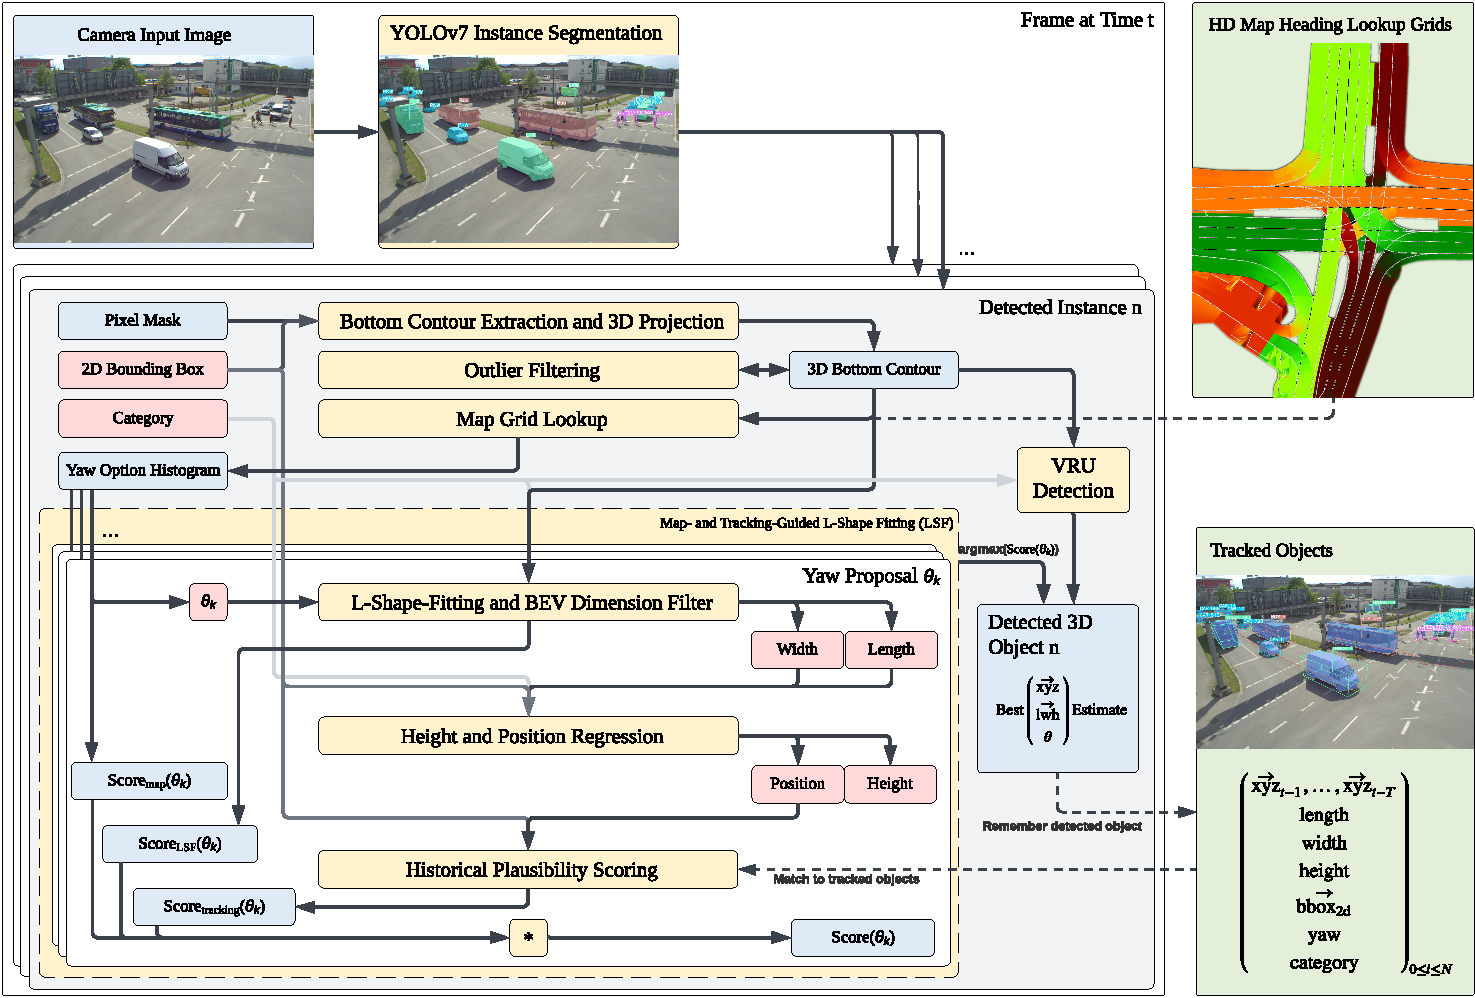
\includegraphics[width=\linewidth]{figures/mono3d-pipeline-lowelevel}
    \caption{Low-level illustration of our \textit{Mono3d} pipeline. To determine a $3D$ pose for a non-VRU $2D$ object instance, its associated pixel mask and category are passed through six processing steps: \textbf{(1)} \textit{Bottom Contour Projection}, \textbf{(2)} \textit{Outlier Filtering}, \textbf{(3)} \textit{Map Grid Yaw Option Lookup}, \textbf{(4)} \textit{L-Shape-Fitting}, \textbf{(5)} \textit{Height and Position Regression}, \textbf{(6)} \textit{Historical Plausibility Scoring}. \textbf{Legend:} Blue boxes mark normal I/O data, red boxes mark I/O variables which are primary components of a final pose hypothesis. Yellow boxes mark processes. Green boxes with dashed arrows mark auxiliary data flow which is not restricted to the scope of the current frame.}
    \label{fig:mono3d-lowlevel}
\end{figure}

The high-level process which turns the instance mask and category inputs into a 3D pose hypothesis for each $2D$ detection is summarized in the following:
First, the instance mask is filtered to extract its bottom contour (see Section~\ref{sec:botcont}).
This yields a line of $2D$ pixel coordinates $\{\overrightarrow{uv}_i\}_{i=0}^{i < N}$.
These are projected back into $3D$ map space using a simple ray-cast, whereas the $z$ (altitude) coordinate is assumed to be 0.
The resulting $3D$ point cloud $\{\overrightarrow{\text{xyz}}_i\}_{i=0}^{i < N}$ is optionally filtered using the \textit{DBSCAN} algorithm to remove outlier points.
If the category of the detected object is that of a \textit{Vulnerable Road User} such as a pedestrian or bicycle, the bottom contour will be converted to a $3D$ pose estimation with a special algorithm as explained in Section~\ref{sec:pedcyc}.
Otherwise, the \textit{HD Map Lookup Grids} (see Section~\ref{sec:hdmapgrids}) are queried at the positions of the $3D$ points.
This query provides a set of $\{(\mathtt{lane\_id}_k, \theta_k)\}_{k=0}^{k<K}$ for each point where the bottom contour touches a particular lane's surface.
These tuples are averaged and aggregated into a histogram per unique \texttt{lane\_id} (see Section~\ref{sec:hdmaplsf}).
This histogram provides $\theta_k$ values with associated confidences $\text{Score}_\text{map}(\theta_k)$ derived from the number of bottom contour points which touch the associated lane.

Thereafter, for each yaw option $\theta_k$, the \textit{L-Shape-Fitting (LSF)} algorithm is used to calculate the physical length and width of the given bottom contour assuming the given $\theta_k$. \textit{LSF} also returns an error score $\text{Score}_\text{lsf}(\theta_k)$ indicating $p(\theta_k|\{\overrightarrow{\text{xyz}}_{0 \leq i < N}\})$ (see Section~\ref{sec:botcontlsf}).
The proposed length and width values are also sanity-checked against limits per the detected object category.
Using these assumed spatial extents, the spatial position and height can be regressed from the $2D$ instance bounding box (see Section~\ref{sec:sizeandpos}).

Finally, the $2D$ instance bounding box is also matched against historical detections via \textit{SORT} object tracking to find previous detections of the same vehicle.
According to the historical vehicle trajectory, a $\theta_k$ proposal also receives a historical plausibility/fitness score $\text{Score}_\text{track}(\theta_k)$ (see Section~\ref{sec:trackinglsf}).
Multiplied together, the three scores $\text{Score}_\text{map}(\theta_k)$, $\text{Score}_\text{lsf}(\theta_k)$ and $\text{Score}_\text{map}(\theta_k)$ yield the final $\text{Score}(\theta_k)$.
Now, for the object in question, we hypothesize that the best $\theta_k$ yaw choice (and associated pose parameters) is the one which finally receives the highest score.
This is calculated for every detected $2D$ object to perform the $2D \rightarrow 3D$ lifting operation.

The following sections of this chapter serve to explain each step in detail.

% ----------------------------------------------------

\section{Bottom Contour Extraction and Filtering}
\label{sec:botcont}

In the first processing step for each $2D$ detection, the detection's pixel mask is converted to a $3D$ bottom contour.
We can express the image mask for detection $n$ as a function $\mathtt{Mask}: \mathbb{N}^2 \rightarrow \mathbb{B}$, as it maps uv pixel coordinates to a boolean value which indicates whether the object occupies the given pixel.
The pixel coordinates are modeled as $\overrightarrow{uv}$ vectors with $u$ indicating the pixel column, $v$ indicating the pixel row, and $\overrightarrow{00}$ as the top-left image corner.
In this model, the $2D$ bottom contour points $B^n_{2D}$ are extracted as follows:

\[
    B^n_{2D}=\{\overrightarrow{uv}|\mathtt{Mask}_n(\overrightarrow{uv}) \land \neg \mathtt{Mask}_n( \begin{pmatrix}u\\v+1\end{pmatrix}) \}
\]

In practice, the operation is realized using a \textit{numpy}~\cite{harris2020array} \textit{argmax} call.
Successively, the $2D$ bottom contour points are projected into $3D$ map space via a raycast operation.
We assume that the ground plane is located at $z=0$, $P$ is the camera's intrinsic (projection) matrix, $R$ is the camera's spatial rotation and $T=\begin{pmatrix} T_x & T_y & T_z \end{pmatrix}$ is the camera's spatial translation relative to the ground plane.
Therefore, the bottom contour $3D$ ground points $B^n_{3D,\text{ground}}$ are calculated as follows:

\begin{gather*}
    B^n_{3D,\text{init}}=\bigcup_{\overrightarrow{uv} \in B^n_{2D}} \{\overrightarrow{\text{xyz}} | \overrightarrow{\text{xyz}} = R^T * P^{-1} * \overrightarrow{uv1}\}\\
    B^n_{3D,\text{ground}}=\bigcup_{\overrightarrow{\text{xyz}} \in B^n_{3D,\text{init}}} \{\overrightarrow{\text{xyz}_\text{ground}} | \overrightarrow{\text{xyz}_\text{ground}} = T + \overrightarrow{\text{xyz}} * -T_z/z\}\\
\end{gather*}

This point set is then filtered using the \textit{DBSCAN}~\cite{schubert2017dbscan} algorithm to get rid of outlier points which do not belong to the true $3D$ bottom outline.

\section{Detection of Vulnerable Road Users}
\label{sec:pedcyc}

\textit{Vulnerable Road Users (VRUs)}, such as pedestrians or bicyclists, receive special treatment in our \textit{Mono3d} pipeline.
This is, because several assumptions which are made for optimized road vehicle detection are not valid for VRUs:

\begin{enumerate}
    \item \textbf{Legal Heading Assumption}: For road vehicles, the monocular detector makes use of the HD map to derive yaw options from legal traffic flow directions.\ This is not possible for bicyclists or pedestrians, as these often move along unmapped territory beyond the road, and perpendicular to normal traffic directions on mapped vehicle lanes.
    \item \textbf{Box Shape Assumption}: Cars, trucks and other motorized road users usually exhibit an instance mask bottom contour shape which indicates the occupied ground area of the object, and therefore allows for L-Shape-Fitting as an effective algorithm to derive the object's length and width.\ This is usually not the case for pedestrians and bicycles, which might have major errors in their back-projected bottom contours (see Figure~\ref{fig:mono3d-vru}).
\end{enumerate}

For these reasons, we have implemented a simplified detection flow for VRUs: We do not attempt to detect their orientation, instead they are always assigned $\theta=0$.
Furthermore, their dimensions are set to fixed values.
The only variables which remain to be estimated are the VRU's BEV coordinates.
This is done by averaging the positions of $10$ percent of the road user's bottom contour $B^n_{3D,\text{ground}}$ points, which are closest to the camera from the BEV perspective.

The reasoning for this strategy is illustrated in Figure~\ref{fig:mono3d-vru}:
The camera $C$ detects pedestrian $A$ and cyclist $B$.
The projection of their instance mask bottom contour (highlighted in red) to the ground is highlighted in blue.
Points on the $3D$ bottom contour which are close to the camera BEV position and therefore considered to estimate the position of $A$ and $B$ are respectively shown.

\begin{figure}[htb]
    \centering
    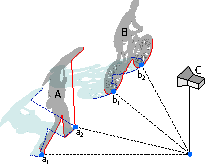
\includegraphics[width=0.8\linewidth]{figures/vru-detection}
    \caption{Illustration of our proposed solution for VRU detection. Camera $C$ observes pedestrian $A$ and cylist $B$. Their 2D bottom contour outline is highlighted in red, the projection of the outline to the ground is highlighted in dashed blue lines. Only the highlighted points on the respective bottom contour projections which remain close to the camera may be considered to estimate the position of $A$/$B$.}
    \label{fig:mono3d-vru}
\end{figure}

\section{Bottom Contour L-Shape Fitting}
\label{sec:botcontlsf}

The process of estimating $\theta$, width and length for motorized road vehicles is realized using the \textit{L-Shape-Fitting (LSF)} algorithm~\cite{zhang2017efficient} with an augmented score calculation function.
From the standard LSF implementation, we use the \textit{Variance} criterion, as it was demonstrated to perform the best in the original paper.
The value of the LSF variance score $\mathtt{Variance}_{\text{LSF}}(\theta_k)$ is in the range of $[-\infty, 0]$.
We normalize this value to the range of $[0, 1]$ as $\text{Score}_\text{lsf}(\theta_k)=1 / (1 - \mathtt{Variance}_{\text{LSF}}(\theta_k))$.
Now, we combine it using multiplication with the map confidence score (see Section~{\ref{sec:hdmaplsf}}) and the historical plausibility score (see Section~{\ref{sec:trackinglsf}}), to arrive at the final  $\text{Score}(\theta_k)$.
Unlike in the original \textit{LSF} algorithm, we constrain the choice of $\theta_k$ to values which are derived from the HD map.

% ----------------------------------------------------

\section{HD Map Lookup Grids}
\label{sec:hdmapgrids}

In this work, we propose to select the $\theta$ heading value for each $3D$ vehicle detection from a traffic flow direction that is derived from the HD map.
However, so far it has been left up to the reader to imagine how the HD map is exactly queried to produce heading options.
The following two sections explain this step in more detail.
First and foremost, we propose a spatial grid lookup structure for heading options at fixed planar increments, covering the \textit{field-of-view (FOV)} of each sensor.
This approach allows us to pre-compute the heading options for a discrete subset of representative map locations, and the subsequent real-time lookup becomes computationally trivial.

\subsection{Lane Tesselation}
\label{subsec:tesselation}

The precise mechanic of rendering the previously outlined heading lookup buffers begins by converting the \textit{OpenDRIVE}~\cite{dupuis2010opendrive} map lane surfaces into triangles.
This process is called \textit{tesselation}.
An \textit{OpenDRIVE} \textit{Road} is defined as a sequence of \textit{Lane Sections} along a reference (center-)line.
A \textit{Lane Section} is a bundle of adjacent lanes.
In the \textit{OpenDRIVE} format, a \textit{Lane} is enclosed between an inner and an outer boundary line.
A \textit{Lane Section} is therefore a sequence of $M+1$ lane boundary lines which enclose $M$ parallel lanes.
We make use of the \textit{OpenDRIVE Converter Tool}~\footnote{\hyperlink{https://github.com/Brucknem-TUMProjects/OpenDRIVE}{https://github.com/Brucknem-TUMProjects/OpenDRIVE}} to sample the \textit{OpenDRIVE} lane boundaries from \textit{Bezier Curves} into polylines.
The tool discretizes the lane boundaries as an array of $\overrightarrow{\text{xyz}}$ coordinates at an interval of one meter.

\begin{figure}[htb]
    \centering
    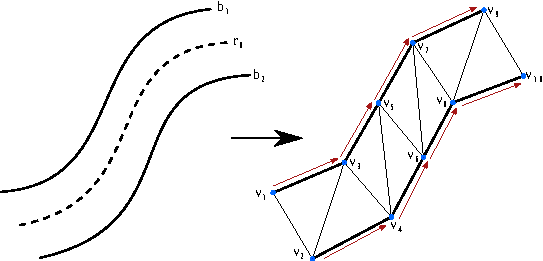
\includegraphics[width=0.8\linewidth]{figures/tesselation}
    \caption{Illustration of our lane tesselation algorithm for a single lane section. The OpenDRIVE lane boundary lines are sampled at constant intervals to convert them to polylines. Orientations are calculated for each derived poly-line vertex. For each lane, the enclosing polylines are then \enquote{zipped} together with a triangle-strip.}
    \label{fig:tesselation}
\end{figure}

As illustrated in Figure~\ref{fig:tesselation}, the result of the lane section point sampling is a matrix $V \in \mathbb{R}^{(M+1) \times N \times 4}$, with $N$ being the number of points sampled along each boundary line.
Each vertex $v_{(m,n)} \in V$ has four scalar components: Three spatial dimensions for its location, and one extra dimension $\theta$ to indicate the heading at its location.
In Figure~\ref{fig:tesselation}, the heading at the vertex position is indicated with a red arrow.
It is calculated as $\theta(v_{(m,n)}) = \mathtt{arctan2}(v_{(m,n+1)} - v_{(m,n)})$.
The last vertex assumes the theta value of the second-to-last.
Each lane $l_m \in \{l_1,\mathellipsis,l_M\}$ is then tessellated as a triangle strip via a sliding window of three vertices over the sequence $\{v_{(m,1)}, v_{(m+1,1)}, \mathellipsis, v_{(m,N)}, v_{(m+1,N)}\} \subseteq V$.
This results in $2(N-1)$ triangles covering the surface of each lane.

\subsection{Lane Rasterization}
\label{subsec:rasterization}

As lanes are converted into batches of triangles, it is possible to use fast rasterization algorithms to \enquote{paint} them into grid buffers.
Rasterization is the process of converting a vector representation of a shape into a pixel or voxel representation.
Both representations have distinct advantages.
A vector representation is usually the most efficient for storage.
But it is comparatively slow to determine whether it contains a specific point, and how that point is situated in relation to the vertices of the geometry.
This is where a pixel or grid-based representation has a lot of potential.
The grid can store which locations are covered by the geometry and can also serve as a cache for vertex attributes of the geometry at each grid cell location.
In case of the lane surfaces, each grid cell stores the heading value of the lane at the grid cell location.
To account for overlapping lanes, we instantiate one grid per \textit{OpenDRIVE} road.
Only lane sections which belong to the same road are rendered into the same grid.

\begin{figure}[htb]
    \centering
    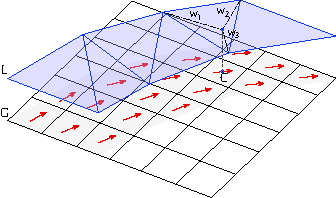
\includegraphics[width=0.7\linewidth]{figures/rasterization}
    \caption{Illustration of lane heading rasterization using barycentric coordinates. Lane $L$ is rasterized into grid $G$, and the barycentric coordinates $w_1$, $w_2$ and $w_3$ are shown for one specific gric-cell center point $C$.}
    \label{fig:rasterization}
\end{figure}

The spatial coverage of each heading lookup grid for a camera is determined by iterating through the available lane sections, and selecting those which are both in view of the camera and not further than 200 meters away.
Each cell in each grid then covers a $10*10$~cm square.
This yields a grid resolution of $898*1140$ cells for the \textit{South-1} camera, and $1436*1224$ cells for the \textit{South-2} camera.
For the highway, we extend the grid range to 1000 meters and increase the grid cell size to $50*50$~cm.

In detail, the process of rasterization means to loop over every \enquote{pixel} (grid cell) and determine if it lies inside one of the triangles of the tessellated lane sections for the road of the tested grid.
If it does, we use the barycentric coordinates of the grid cell with respect to the triangle to interpolate the corresponding heading value for the point inside the triangle.
This process is also illustrated in Figure~\ref{fig:rasterization}.

The algorithm involves the following steps:

\begin{enumerate}
    \item Given a triangle with vertices $v_1$, $v_2$, and $v_3$, and a grid with width $w$ and height $h$, loop over every cell which is within the bounding box of the triangle.
    \item For each candidate cell $C=(x,y)$, compute the barycentric coordinates $(w_1, w_2, w_3)$ of the cell with respect to the triangle using the following formulas:

    \[
    \begin{aligned}
    \vec{v_1v_2} &= \vec{v_2} - \vec{v_1} \\
    \vec{v_1v_3} &= \vec{v_3} - \vec{v_1} \\
    \vec{v_1c} &= C - \vec{v_1} \\
    w_1 &= \frac{\vec{v_1v_3} \times \vec{v_1c}}{\vec{v_1v_3} \times \vec{v_1v_2}} \\
    w_2 &= \frac{\vec{v_1c} \times \vec{v_1v_2}}{\vec{v_1v_3} \times \vec{v_1v_2}} \\
    w_3 &= 1 - w_1 - w_2
    \end{aligned}
    \]

    Note that the order of the vertices in the cross product determines the winding order of the triangle.\ If the winding order of the triangle is reversed, the signs of the cross products will also be reversed.

    \item If all three barycentric coordinates are non-negative, the pixel lies inside the triangle.\ We can then use the barycentric coordinates to interpolate the corresponding heading value $\theta_C$ of the grid cell $C$ inside the triangle using the following formula:

    \[
    \begin{aligned}
    \theta_C &= w_1 \theta(\vec{v_1}) + w_2 \theta{v_2} + w_3 \theta(\vec{v_3}) \\
    \end{aligned}
    \]

    where $\theta(\vec{v})$ is the heading for a boundary vertex as described in Section~\ref{subsec:tesselation}.

    \item Repeat steps 1--3 for every grid cell of every road grid.

\end{enumerate}

In practice, we have implemented this algorithm in \textit{numpy}, which allows the parallel execution of all grid cell tests for one triangle.
A triangle covers $99.85$ cells on average.
This makes the process of rendering the heading lookup grids quite fast, with an average wall-time of $1.48s$ to render $6812$ triangles on a Ryzen 5600 processor.
This process can be comfortably executed during the startup of the $3D$ detector process.
At an average of 25 \textit{OpenDRIVE} roads per camera view on the S110 intersection, and five bytes stored per cell, the final grid-set for one camera occupies $165.78 MiB$ of RAM on average.
The resulting heading fields are visualized in Figure~\ref{fig:headings-rendered}.

\begin{figure}[htb]
    \centering
    \includegraphics[width=0.49\linewidth]{figures/headings-s2}
    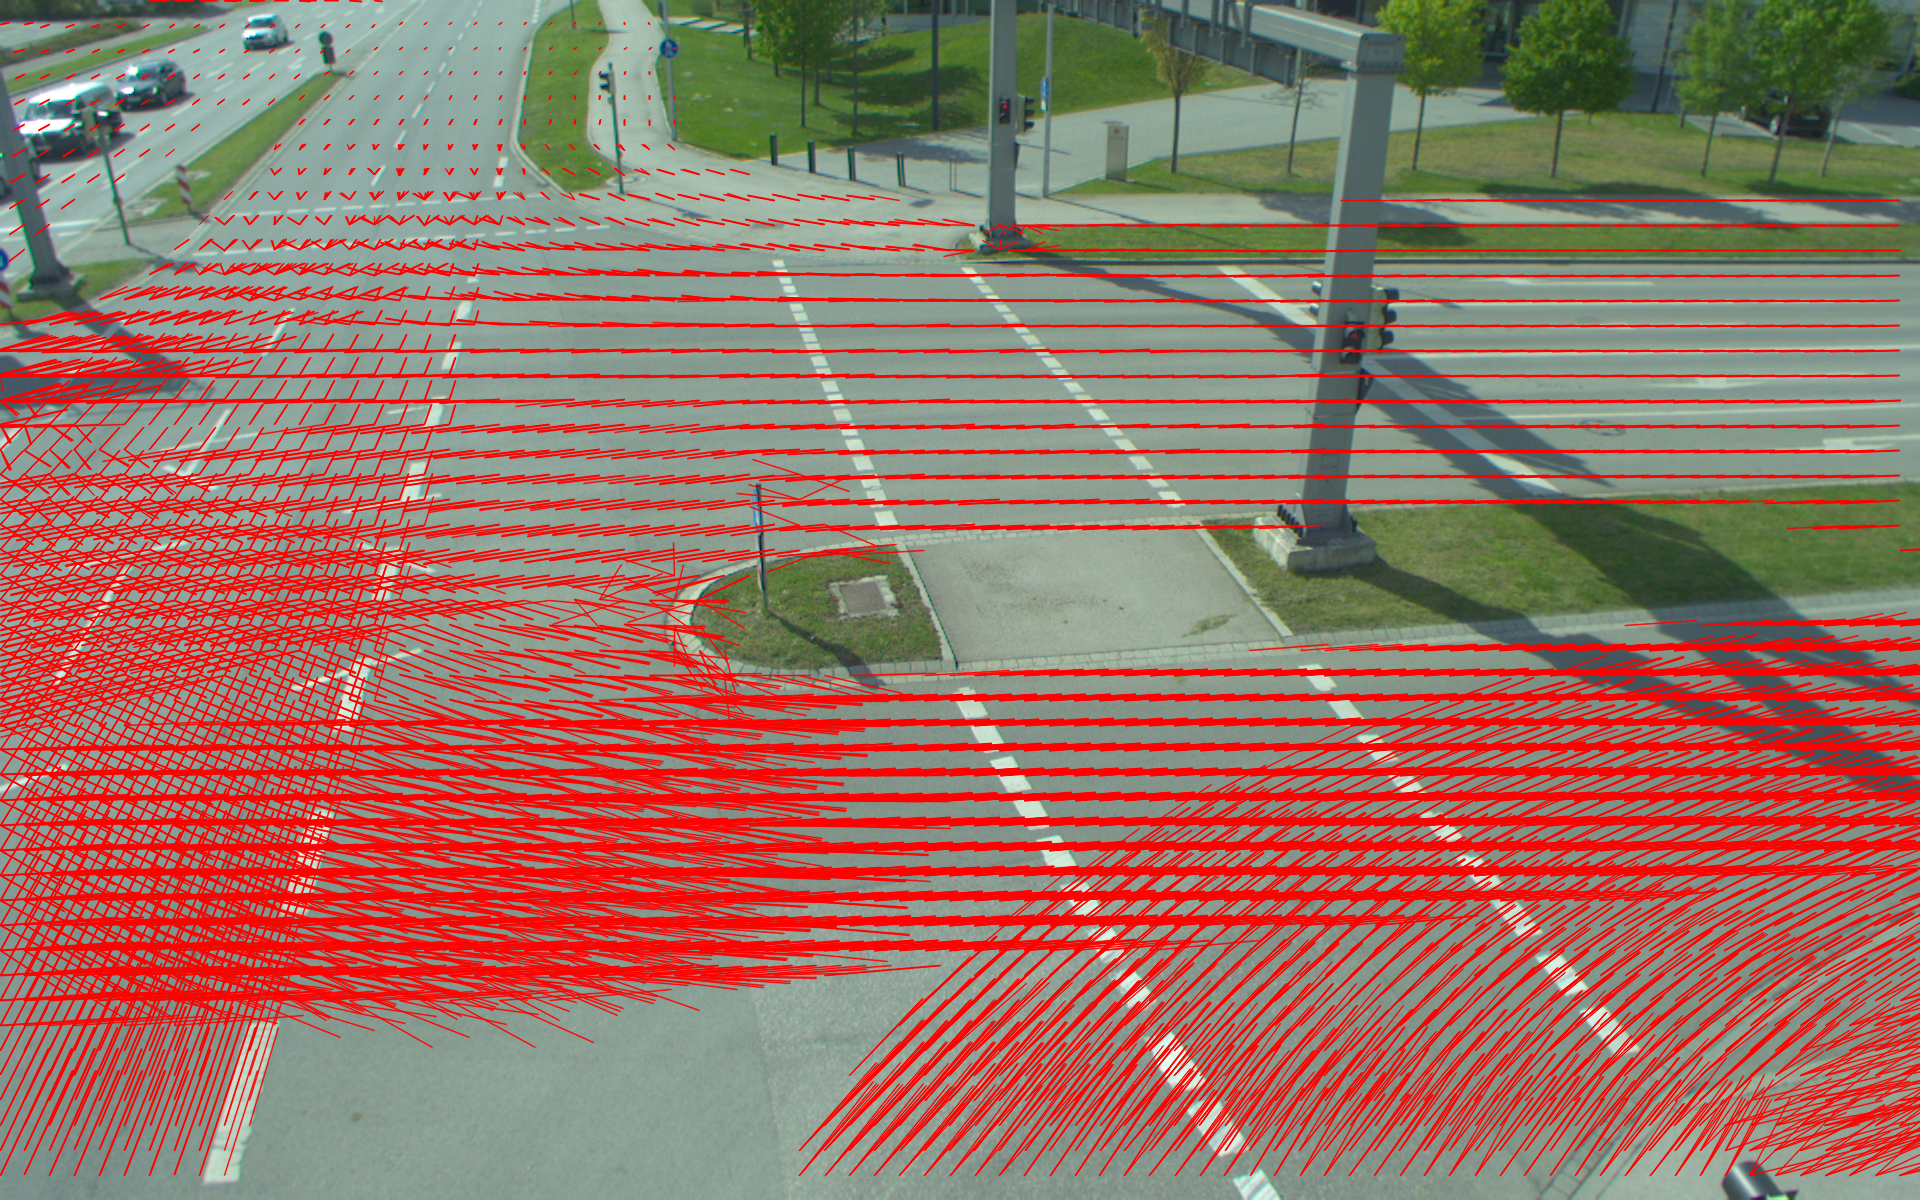
\includegraphics[width=0.49\linewidth]{figures/headings-s1}
    \caption{Derived heading values rendered on top of the S110-S2 camera perspective (left) and the S110-S1 camera perspective (right).}
    \label{fig:headings-rendered}
\end{figure}

% ----------------------------------------------------

\section{HD-Map-Augmented L-Shape Fitting}
\label{sec:hdmaplsf}

The previously outlined heading lookup grids, which are rendered from the HD map, can improve the basic LSF algorithm in two ways:

\begin{enumerate}
    \item The grid may be used to calculate possible heading values which are to be evaluated by LSF, rather than using the basic approach of iterating over $[0, \pi]$ at fixed increments.
    \item The grid can also yield a confidence value $\text{Score}_\text{map}(\theta_k)$ for each heading option $\theta_k$, given how many bottom contour points support the respective option.
\end{enumerate}

In general, the heading lookup grids $G_1,\mathellipsis,G_{|R|}$ for each road $r \in R$ are queried using the bottom contour $B^n_{3D}$ of vehicle detection $n$, which is a series of $3D$ points $\overrightarrow{\text{xyz}^n_1},\mathellipsis,\overrightarrow{\text{xyz}^n_k}$.
We define the grid lookup operator $G_r(\overrightarrow{xy})$ as a function $\mathbb{R}^2 \rightarrow \mathbb{B} \times \mathbb{R}$ which delivers a boolean flag and a heading value given an arbitrary planar bottom contour position.
The boolean flag indicates whether the road $r$ covers the position $\overrightarrow{xy}$ at all.
The two return values of the operator are referenced as $G_r(\overrightarrow{xy})_\mathbb{B}$ and $G_r(\overrightarrow{xy})_\theta$, respectively.

Now, the confidence of the map that a particular road grid $G_r$ provides the correct heading for detection $n$ may be expressed through the absolute count of bottom contour points $\overrightarrow{\text{xy}^n_i} \in B^n_{3D}$ for which $G_r(\overrightarrow{xy}^n_i)_\mathbb{B}$ is true.
We call this count the \textit{lookup histogram value} $h(G_r,B^n_{3D})$ for the road grid $G_r$ and the bottom contour $B^n_{3D}$.
The heading option $\theta_r$ provided by $G_r$ will then be the $\mathtt{average}(\{G_r(\overrightarrow{xy}^n_i)_\theta|G_r(\overrightarrow{xy}^n_i)_\mathbb{B}\}_{i=1}^{i \leq k})$.
Finally, the lookup histogram value must be converted to a range of $[0,1]$ to become a score which can be used as a factor.
To this end, we normalize $h(G_r,B^n_{3D})$ as $\text{Score}_\text{map}(\theta_r, B^n_{3D})$:

\[
    \text{Score}_\text{map}(\theta_r, B^n_{3D})=\frac{h(G_r,B^n_{3D})}{\max_{s \in R} h(G_s,B^n_{3D})}
\]

This process is illustrated in Figure~\ref{fig:mapscore}.
There are three grids $G_1$, $G_2$ $G_3$ for three overlapping roads.
The bottom contour of vehicle $V$ as observed by camera $C$ is shown with 11 points.
Now, the lookup histogram values for each grid are shown in the bar-chart on the right side of the figure.
For grid $G_1$, all 11 points match to a nonempty cell.
For grid $G_2$, six points match.
For grid $G_3$, only five points match.
These absolute histogram values are then converted to relative confidence score values, by dividing each over the maximum histogram value, which is 11.

\begin{figure}[htb]
    \centering
    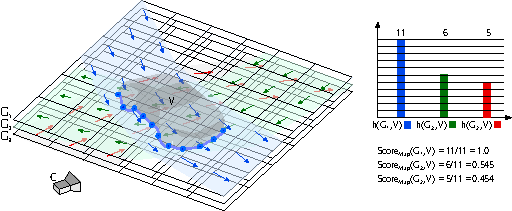
\includegraphics[width=1.0\linewidth]{figures/mapscore}
    \caption{Illustration of a map heading histogram lookup for the bottom contour of vehicle $V$. The map lookup grid-set provides grids for three roads $G_1$, $G_2$ and $G_3$. The histogram values $h(G,V)$ per road, as well as the respective normalized scores which are calculated from the histogram, are shown on the right.}
    \label{fig:mapscore}
\end{figure}


% ----------------------------------------------------

\section{Tracking-Augmented L-Shape Fitting}
\label{sec:trackinglsf}

In the example from Figure~\ref{fig:mapscore}, the vehicle is conveniently positioned such that the correct heading option clearly wins the highest confidence score.
However, it is easily possible to imagine $V$ in a position slightly further upwards, where the map confidence scores would not be so unambiguous.
For such cases, the raw LSF variance criterion score may help.
However, we hypothesize that the vehicle's positional history, as described all the way back in the Introduction Section~\ref{subsec:sstracking} may provide an additional historical plausibility score $\text{Score}_\text{track}(\theta_k, V)$ for vehicle $V$ and heading candidate $\theta_k$.

This is calculated as follows: Using a screen-space SORT tracker~\cite{bewley2016simple}, we match a detected object's bounding box to detections from previous frames.
For a successfully matched detection, historical 3D position values $L=\{\vec{l}_{t-1},\dots,\vec{l}_{t-T}\}$ are retrieved.
Given the historical positions $L$ and a position hypothesis $\vec{l}_t(\theta_t)$, the historical plausibility score $\text{Score}_\text{track}(\theta_k, V)$ for a yaw hypothesis $\theta_k$ is calculated as in the following equation:

\[
    \text{Score}_\text{track}(\theta_k, V)=\prod_{\delta_t=1}^{\delta_t \leq T}\pi/2 - \Delta_\angle(|\theta_{t} - \text{atan2}(\vec{l}_t(\theta_t)-\vec{l}_{t-\delta_t})| \mathtt{~mod~}\pi)
\]

The Delta-Angle function $\Delta_\angle: [0, \pi) \rightarrow [0, \pi/2)$ converts the passed raw angular difference, which is already less than $\pi$, into a value less than $\pi/2$ by returning angular deltas $\delta_{>\pi/2}$ larger than $\pi/2$ as $\pi-\delta_{>\pi/2}$.
This ensures that a yaw hypothesis, which is parallel, yet opposed to a historical orientation, is not erroneously punished.
In practice, we have implemented a threshold of six historical positions that are evaluated to determine the plausibility of a yaw hypothesis.

% ----------------------------------------------------

\section{Joint Height and Position Estimation}
\label{sec:sizeandpos}

As an estimate for a detected vehicle's width and length is made using our augmented L-Shape-Fitting algorithm, two critical values remain to be established for a fully defined 3D bounding box: The vehicle position and the vehicle height.
Also, our tests showed that the LSF-based BEV dimension hypothesis must often be corrected due to errors in the bottom contour (see Sections~\ref{sec:impactcontourfiltering} and~\ref{sec:impactcontourfiltering}).
Because of this, we need to clamp the BEV width/length dimensions to category-based minimum and maximum values.
In this case, the vehicle's bounding box needs to grow or shrink in some direction, and the position hypothesis of the LSF algorithm becomes uncertain.

\begin{figure}[htb]
    \centering
    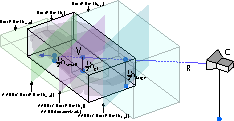
\includegraphics[width=1.0\linewidth]{figures/calc-height-pos}
    \caption{Illustration of a joint 3D height and location for vehicle V. Initially, camera $C$ observes only the screen-space bounding box $\mathtt{AABB}(\texttt{InstanceMask}_V)$.\ We now search for the vehicle height $h$ based on a value along the ray $R$, which is cast from $C$ through the 2D AABB center.\ Only for the correct $h_\text{gt}$ will the 2D AABB of the predicted 3D box $\mathtt{AABB}(C,\mathtt{Box}(R,w,l,\theta,h_\text{gt}))$ be equal to $\mathtt{AABB}(\texttt{InstanceMask}_V)$.}
    \label{fig:calcheightpos}
\end{figure}

There is however a strong criterion towards the position of the 3D bounding box, which we can use to estimate it: It is desirable to position a vehicle's 3D bounding box such that it covers the 2D instance mask of the same vehicle when projected to screen-space.
This also means, that the screen-space-projected center of the 3D bounding box should coincide with the center of the 2D bounding box.
So we know, that the center of the 3D bounding box must be somewhere along a 3D ray which is cast from the camera through the center of the instance mask.
Because a camera mounted from the infrastructure perspective also generally looks down, the position along the ray also dictates the height (more specifically half of the height) of the vehicle.
Now, as the bounding box height changes, so does the height of its 2D screen-space projection.
Therefore, we can simultaneously optimize both the height of the 3D box and its position, with the goal to match the screen-space bounding box of the estimated 3D bounding box to the instance mask bounding box.

\begin{algorithm}
\caption{RegressHeightAndLocation}\label{alg:posheightregression}
\begin{algorithmic}[1]
\Require $\texttt{width}, \texttt{length}, \texttt{theta}, \texttt{bbox\_2d}, \texttt{cam}, \texttt{min\_height}, \texttt{mean\_height}, \texttt{max\_height}$
\Ensure $\texttt{height}, \texttt{location}$
\State $\texttt{x0, y0, x1, y1} \gets \texttt{bbox\_2d}$
\State $\texttt{detection\_img\_height} \gets \texttt{y1} - \texttt{y0}$
\State $\texttt{height} \gets \texttt{mean\_height}$
\Comment{Initially estimate height by mean for category}
\State $\texttt{jump\_size} \gets \texttt{max\_height} - \texttt{mean\_height}$
\State $\texttt{mask\_center} \gets \begin{bmatrix}
\texttt{x0} + (\texttt{x1} - \texttt{x0})//2 \
\texttt{y0} + (\texttt{y1} - \texttt{y0})//2
\end{bmatrix}$
\State $\texttt{location} \gets \begin{bmatrix}
0 \
0 \
0
\end{bmatrix}$
\For{$\texttt{i} \gets 0$ to $9$}
\Comment{Binary search for correct height/position, 10 iterations max.}
\State $\texttt{location} \gets \texttt{cam.project\_to\_ground}(\texttt{mask\_center}, \texttt{height} \times 0.5)$
\State $\texttt{location[2]} \gets 0$
\State $\texttt{box} \gets \texttt{get\_box}(\texttt{theta, width, length, location})$
\State $\texttt{box} \gets \texttt{box} \oplus (\texttt{box}+\begin{bmatrix}
0 & 0 & \texttt{height}
\end{bmatrix})$
\State $\texttt{all\_corners\_projected} \gets \texttt{cam.project\_to\_image}(\texttt{box}^\top)$
\State $\texttt{min\_img\_y} \gets \min(\texttt{all\_corners\_projected[1]})$
\State $\texttt{max\_img\_y} \gets \max(\texttt{all\_corners\_projected[1]})$
\State $\texttt{estimated\_img\_height} \gets \texttt{max\_img\_y} - \texttt{min\_img\_y}$
\State $\texttt{img\_height\_delta} \gets \texttt{detection\_img\_height} - \texttt{estimated\_img\_height}$
\If{$|\texttt{img\_height\_delta}| < 1.0$}
\Comment{Less than one px difference. We are done.}
\State \textbf{break}
\EndIf
\If{$\texttt{i} > 0$ \textbf{and} $\texttt{sign(img\_height\_delta)} \neq \texttt{sign(jump\_size)}$}
\State $\texttt{jump\_size} \gets \texttt{jump\_size} \times 0.5$ \Comment{Halve the step size on direction change.}
\EndIf
\State $\texttt{jump\_size} \gets \texttt{sign(img\_height\_delta)} \times |\texttt{jump\_size}|$
\State $\texttt{prev\_height} \gets \texttt{height}$
\State $\texttt{height} \gets \texttt{height} + \texttt{jump\_size}$
\State $\texttt{height} \gets \max(\min(\texttt{height}, \texttt{max\_height}), \texttt{min\_height})$ \Comment{Respect limits.}
\If{$\texttt{height} = \texttt{prev\_height}$} \Comment{We've hit a limit, no need to continue iterating.}
\State \textbf{break}
\EndIf
\EndFor
\State \Return $\texttt{height}, \texttt{location}$
\end{algorithmic}
\end{algorithm}

In practice, we have implemented this joint height and position regression using binary search over the 3D height value, as described in Algorithm~\ref{alg:posheightregression}.
As the optimization goal, it is sufficient to match the image space box height.
We limit the number of optimization steps to 10, but observe that the algorithm converges on average after five steps.
We also add a sanity check to abort iteration, if the optimization cannot progress because the estimated height is growing below or beyond sanity limits.
This can occur when the pixel mask for the detected instance is highly erroneous or obscured.
The approach is also illustrated in Figure~\ref{fig:calcheightpos}.
Initially, camera $C$ observes only the screen-space bounding box $\mathtt{AABB}(\texttt{InstanceMask}_V)$.\ We now search for the vehicle height $h$ based on a value along the ray $R$, which is cast from $C$ through the 2D AABB center.\ Only for the correct $h_\text{gt}$ will the 2D AABB of the predicted 3D box $\mathtt{AABB}(C,\mathtt{Box}(R,w,l,\theta,h_\text{gt}))$ be equal to $\mathtt{AABB}(\texttt{InstanceMask}_V)$.

% ----------------------------------------------------

\section{Late HD Map Lookup}
\label{sec:hdmaplate}

In the rest of this chapter, two optional design elements are explained which do not necessarily improve our system, but answer some questions in our evaluation study.
Feel free to skip ahead to the next chapter if you are only interested in the best version of the system.

First, as an alternative to the rather complex \enquote{early} HD map lookup for all bottom contour points (with a derived confidence histogram which feeds into L-Shape-Fitting), we initially also implemented much a simpler \enquote{late lookup} approach.

Here, we only query the HD map for heading options at the current vehicle position.
Then we pick the heading option which is most in line with the vehicle's historic positions, or merely the option closest to the LSF-based proposal, if tracking is turned off.

The drawbacks of this approach are manifold: L-Shape-Fitting has already settled on a heading value prior to the map lookup, so the width and length will not be corrected.
Furthermore, the vehicle position at this point is already very disconnected from the ground-truth sensor input.
So, a lot of positional information is discarded before the HD map lookup is made.
Finally, the joint position-height regression algorithm relies on established values for width, length and $\theta$, so correcting $\theta$ afterwards is logically not optimal.

\section{3D SORT Tracking}
\label{sec:trackthreed}

Another \enquote{questionable idea} (in hindsight) which we tested was to use \textit{SORT} in 3D bird's-eye-view (BEV).
In conjunction with 2D screen-space tracking, which is required to calculate the historical plausibility score for L-Shape-Fitting, we have also applied the \textit{SORT} algorithm to track detections in 3D BEV space.
This is supposed to stabilize 3D position estimates through the \textit{Kalman Filters} which are used by \textit{SORT}.
Because \textit{SORT} does not support a heading value in the bounding box state, we feed BEV detections as squares of size $((l+w)/2)^2$ into the algorithm.
This is immediately obvious as a drawback of using \textit{SORT} for 3D tracking, and we do not expect this application of \textit{SORT} to improve our results.
Instead, a more capable Kalman Filter detection is needed which also takes vehicle heading into account.
